
\chapter{Metody pro~hledání bodových odhadů}\label{kapitola2}


\section{Metoda momentů}
Tato metoda je založená na~užití výběrových momentů, ať už centrálních nebo necentrálních, případně i~z~momentů rozdělení. V~praxi pak využijeme tu, která se~dá vypočítat nejjednodušeji.
V této metodě bereme v~potaz všechny realizace.

Máme tedy $\prostor,~\t\in\Theta\subset\R^k,~\tau(\t)$ jako odhadovanou parametrickou funkci, vlastnost $X~iid~f_X(x,\t)$. Nechť $X_1,...,X_n~iid~\LL_k$ (aby existovaly momenty do~řádu $k$) a~označíme \[
\begin{split}
\mu_r&=\mu_r(\t)=\E X^r,~r\in\hat{k},\\
\bmu(\t)&=\br{\mu_1(\t),...,\mu_k(\t)}:\R^k\to\R^k.
\end{split}
\]
Dále požadujeme, aby $\exists\bmu^{-1}$, tedy například aby $\bmu$ bylo regulární a~prosté. 

\begin{define}[Momentový odhad]
	\textbf{Momentový odhah} $\t$ definujeme vztahem
	$$ \htm:=\htm(\X)=\bmu^{-1}\br{m'_1(\X),...,m'_k(\X)}\text{,\quad  kde }m'_r(\X)=\frac{1}{n}\sumjn X_j^r, $$ což znamená, že $\htm$ je řešením \textit{soustavy momentových rovnic} (značíme $ME_q$) ve~tvaru $$\mu_r(\t)=m'_r(\X),\quad \forall r \in\hat{k}.$$ Definujeme dále \textbf{momentový odhad} $\tau(\t)$ vztahem $T_\txt{M}(\X):=\tau\br{\htm(\X)}$, metoda momentů je tedy invariantní na~transformace parametru $\t$ (je to jen jiné vyjádření pro~vztah\\ $T_\txt{M}(\X)=\widehat{\tau(\t)_\txt{M}}=\tau(\htm)$).
\end{define}
\begin{remark}
	\begin{enumerate}
		\item Pokud soustava $ME_q$ není jednoznačně řešitelná, případně některý z~momentů $\mu_r$ nezávisí na~$\t$, pak můžeme přidat další rovnici ve~tvaru $\mu_{k+1}(\t)=m_{k+1}(\X)$.
		\item Alternativně lze užít i~centrální momenty
		$$ \mu_r(\t)=\E(X-\E X)^r,\qquad m_r(\X)=\frac{1}{n}\sumjn (X_j-\Oxn)^r. $$
	\end{enumerate}
\end{remark}
\begin{example}
	Mějme $\poslkon~iid~\NN(\mu,\sigma^2)$. Pak je soustava $ME_q$ ve~tvaru \[
	\begin{split}
	\E X&=\mu\stackrel{!}{=}\Oxn, \\ \E(X-\E X)^2&=\D X=\sigma^2\stackrel{!}{=}\frac{1}{n}\sumjn (X_j-\Oxn)^2=\hsn.
	\end{split}
	\] Momentové odhady $\widehat{\mu}_\txt{M} = \Oxn$ a~$\widehat{\sigma}^2_\txt{M}=\hsn$ jsou tedy konzistentní a~$\AN$ odhady $\mu$ a~$\sigma^2$. Obecně však momentové odhady nejsou eficientní.
\end{example}
\begin{theorem}
	Pokud je $\inv{\bmu}$ spojitá funkce, pak $\htm(\X)$ je \textbf{konzistentním} odhadem $\t$. Pokud je navíc $\tau$ spojitá, pak $T_\txt{M}(\X)$ je konzistentní.
	\begin{proof}Ze ZVČ (Chinchin) víme, že 
		$m_1(\X)\PSJ\mu_1,...,m_k(\X)\PSJ\mu_k$. Pak ale
		$$
		\htm=\inv{\bmu}\br{m_1(\X),...,m_k(\X)}\PSJ\inv{\bmu}(\mu_1,...,\mu_k)=\inv{\bmu}(\bmu(\t))=\t.$$
		Podobně pak $T_\txt{M}(\X)=\tau(\htm)\PSJ\tau(\t)$ pro~$\tau(\t)$ spojité.
	\end{proof}
\end{theorem}

\begin{remark}[Připomínka Delta metody] Mějme $\poslnn$ do~$\R^k,~\X_n\sim\AN_k\br{\theta,\frac{1}{n}\C(\theta)}$. Nechť $g:\R^k\to\R$ je borelovská, $\nabla g(\theta)\neq 0,~\exists\frac{\partial g}{\partial\theta_i}$ na~$H_\theta$ (okolí $\theta$) a~jsou spojité v~bodě $\t$. Pak $$ g(\X_n)\sim\AN_1\Br{g(\theta),\frac{1}{n}\nabla g(\theta)\C(\theta)\nabla g(\theta)^T}. $$
	Zobecnění pro~$g:\R^k\to\R^k$: Pokud Jacobiho matice $\mathbb{J}_g$ zobrazení $g$ existuje na~okolí $H_\t$ a~je spojitá v~bodě $\t$, $\mathbb{J}_g(\t)\neq \textbf{0}$, pak
	$$ g(\X_n)\sim\AN_k\Br{g(\t),\frac{1}{n}\mathbb{J}_g(\t)\C(\t)\mathbb{J}_g(\t)^T}. $$
\end{remark}

\begin{theorem}
	Nechť $\htm$ je odhad metodou momentů, $\posl\in\LL_{2k},~\bmu$ je difeomorfismus $(\bmu,\inv{\bmu}$ spojitě diferencovatelné$)$. Pak $\forall\t\in\Theta$ je $$\htm\sim\AN\Br{\t,\frac{1}{n}\C_\txt{M}(\t)},$$ kde $\C_\txt{M}(\t)=\mathbb{J}_{\inv{\mu}}(\t)\C(\t)\mathbb{J}_{\inv{\mu}}(\t)^T$ a~$\C=\Cov(X,X^2,...,X^k)$.  Pokud je navíc $\tau(\t)$ spojitě diferencovatelné a~$\nabla\tau(\t)\neq0$, pak $$T_\txt{M}(\X)\sim\AN\br{\tau(\t),\frac{1}{n}\nabla\tau(\t)\C_\txt{M}(\t)\nabla\tau(\t)^T}.$$
	\begin{proof}
		Definujeme $\mathbb{Z}_j:=(X_j,X_j^2,...,X_j^k)$. Potom
		$$ \E \mathbb{Z}_j=(\E X_j,\E X_j^2,...,\E X_j^k)=(\E X,\E X^2,...,\E X^k)=\bmu(\t). $$
		Označme nyní $\Cov (\mathbb{Z}_j)=\Cov(X,X^2,...,X^k)=\C(\t)$. Víme, že $\mathbb{Z}_j~iid~\LL_2$, tudíž dle CLT v~$\R^k$ platí, že $\overline{\mkern-1mu \mathbb{Z}_n \mkern-3mu}=\br{m_r(\X)}_{r=1}^k\sim\AN_k\br{\bmu(\t),\frac{1}{n}\C(\t)}$. Pak pro~$g=\inv{\bmu}$ spojitě diferencovatelné dostáváme z~$\Delta$-metody vztah
		$$ \htm=\inv{\bmu}\Br{\br{m_r(\X)}_{r=1}^k}\stackrel{\ref{lamatko}}{\sim}\AN\Br{\t,\frac{1}{n}\underbrace{\mathbb{J}_{\inv{\mu}}(\t)\C(\t)\mathbb{J}_{\inv{\mu}}(\t)^T}_{\C_\txt{M}(\t)}}. $$
		Následně pro~$\tau$ spojitě diferencovatelné opět z~$\Delta$-metody dostaneme, že
		$$ T_\txt{M}(\X)=\tau(\htm)\sim\AN\Br{\tau(\t),\frac{1}{n}\nabla\tau(\t)\C_\txt{M}(\t)\nabla\tau(\t)^T}. $$
	\end{proof}
\end{theorem}
\begin{example}
	Mějme $X_1,...,X_n~iid~\n{\mu,\sigma^2}$, kde neznáme hodnotu parametrů $\mu$ a~$\sigma^2$. Víme ale, že 
	$$ \E X_i=\mu,\quad \D X_i=\sigma^2\text{\quad a\quad }\E (X_i)^2=\D X_i+(\E X_i)^2=\sigma^2+\mu^2. $$
	Odhady parametrů metodou momentů dostaneme z~rovnic
	$$ \mu=m_1'=\Oxn\text{\quad a\quad }\sigma^2=m_2 =\frac{1}{n}\br{\sumjn X_j-\Oxn}^2=\hsn. $$
	Tím získáme odhady $\widehat{\mu}_\txt{M},~\widehat{\sigma}_\txt{M}^2$.
\end{example}
\section{Nestranné odhady s~minimálním rozptylem (UMVUE)}

\begin{define}
	Mějme $X_1,...,X_n~iid~\FF,~\t\in\Theta\subset\R^k,~\tau(\t)\in\R^1,~T(\X)$ jako odhad $\tau(\t)$. Definujeme $$T_{\txt{UMR}}=\argmin\limits_T \E\br{T(\X)-\tau(\t)}^2,\quad\forall\t\in\Theta.$$
	Definujeme dále kvadratickou \textbf{ztrátovou funkci} (\textit{loss function}) jako $$\Loss_2(T,\t):=\br{T(\X)-\tau(\t)}^2$$
	a příslušnou \textbf{rizikovou funkci} (\textit{risk function}) vztahem $$R(T,\t):=\E \Loss_2(T,\t).$$ Potom $T_{\txt{UMR}}=\argmin\limits_TR(T,\t)$, kde
	UMR je zkratka pro~\textit{uniformly minimum risk}. $T_{\txt{UMR}}$ je tedy odhad, který minimalizuje hodnotu rizikové funkce $R$.
\end{define}
\begin{define}
	$S(\X)$ se~nazývá \textbf{postačující statistika} (\textit{sufficiency}) pro~$\t$, pokud rozdělení $\X$ podmíněné hodnotou $S(\X)=s$ nezávisí na~parametru $\t$. Pro~diskrétní případy tedy\newline $\PP(\X=\textbf{x}|S(\X)=s)$ nezávisí na~$\t$, případně $f_{\X | S}(\textbf{x}|s)$ nezávisí na~$\t$.
	\\ \\
	Postačující statistika je tedy taková funkce náhodného výběru (statistika), která umí sama o~sobě nahradit původní výběr bez~ztráty informace o~parametru $\t$.
\end{define}
\begin{example}
	Házíme mincí, $X_i\sim\Be(\t)$, $\textbf{x}=(0,1,1,0,1,...)$. Představme si, že chceme vypočítat tzv. MLE (bude definováno později) ve~tvaru $$ L=\prod\limits_{i=1}^N \t^{x_i}(1-\t)^{1-x_i}\qquad=\t^{x_1+x_2+...}(1-\t)^{1-x_1+1-x_2+...}=\t^{\sm{i=1}{N}x_i}(1-\t)^{N-\sm{i=1}{N}x_i}. $$
	Pak ale ve~výsledku nezáleží na~samotných datech, ale pouze na~jejich součtu, tedy pokud označíme $S(\X):=\sm{i=1}{N}X_i$, pak $S(\X)$ je postačující statistika (podle Neymannova fatrorizačního kritéria).
	%https://www.youtube.com/watch?v=5j4E2FRR384
\end{example}
\begin{define}	Mějme $X,Y$ náhodné veličiny na~$\prostor$. Pak $$\E(X|Y=y)=\int\limits_{\R} x\d \PP^{X|Y=y}=\Big[\text{pro ASR }f_{X|Y}(x|y):=\frac{f_{X,Y}(x,y)}{f_Y(y)}\Big]=...$$
	Z toho vyplývá, že $\E(X|Y):\Omega\to\R$ je náhodná veličina.
\end{define}

\begin{theorem}
	Pro náhodné veličiny $(X,Y)$ s~ASR $f_{X,Y}$ platí vztah
	$$ \E\big[\E(X|Y)\big]\equal{\text{ASR}}\int\limits_{\R} \Br{\int\limits_{\R} xf_{X|Y} \d x} f_Y\d y \equal{\text{F.V.}}\int\limits_{\R}\Br{\int\limits_{\R} f_{X|Y}f_Y\d y}x\d x=\int\limits_{\R}\Br{\int\limits_{\R} f_{X,Y}\d y}x\d x=\int\limits_{\R} xf_X\d x=\E X. $$	
\end{theorem}
 ~\\
Pro účely následující Rao-Blackwellovy věty označme $$T_{\txt{RB}}(\X)=T_{\txt{RB}}\br{S(\X)}:=\E\big[ T(\X)|S(\X)=s \big]$$ za~předpokladu existence $\E$ jako odhad zkonstruovaný v~Rao-Blackwellově větě. 
$T_{\txt{RB}}(\X)$ je tedy opět statistika, pro~kterou platí, že $$ T_{\txt{RB}}(\X):=\E\big[ T(\X)|S(\X)=s \big]\equal{\text{ASR}}\int T(\textbf{x})f_{T(\X)|S(\X)=s} \d \textbf{x}.$$
Na $T_\txt{RB}(\X)$ pohlížíme jako na~funkci $\X$, která vznikne ve~dvou krocích:\begin{enumerate}
		\item spočítá se~podmíněná střední hodnota $\E\br{T(\X)|S(\X)=s}=T(s)$ při~libovolně daném pevném $s$,
		\item za~$s$ se~dosadí vazba $s=S(\X)$, čímž vznikne $T_\txt{RB}\br{S(\X)}$.
	\end{enumerate}


\begin{theorem}[Rao-Blackwell]
		Mějme $X_1,...,X_n~iid~\FF,~\t\in\Theta\subset\R^k,~\tau(\t)\in\R^1,~T(\X)$ jako odhad $\tau(\t)$, nechť $S(\X)$ je postačující statistika pro~$\t$ a~nechť $\Loss(T,\t)$ je konvexní funkcí v~$T$ pro~$\forall\t\in\Theta$.
	Pak $$R\br{T_{\txt{RB}}(\X),\t}\leq R\br{T(\X),\t},\quad\forall\t\in\Theta,$$ přičemž $T_{\txt{RB}}$ nezávisí na~$\t$. 
\begin{proof}Větu ukážeme obecněji pro~$\Loss(T,\t)$ konvexní v~$T$, která zahrnuje i~naši kvadratickou ztrátovou funkci $\Loss_2$. Pro~$\forall\t\in\Theta$ z~Jensenovy nerovnosti platí, že
	$$R(T_{\txt{RB}},\t)=\E \Loss\br{\EE{T| S=s},\t}\leq\E\big[ \EE{\Loss(T,\t)|S=s} \big]=\E \Loss(T,\t)=R(T,\t).$$
\end{proof}
\end{theorem}
\begin{define}
	Systém hustot $\mathcal{F}=\mathcal{F}_X=\{ f(x,\t):\t\in\Theta\subset\R^k \}$ se~nazývá \textbf{úplný}, pokud pro~
	$\forall h:\R\to\R,~\E_\t h(X)=0,~\forall\t\in\Theta$ platí, že$$ h(X)=0~s.j.\quad \forall\t\in\Theta,\quad \text{neboli}\quad \PP_\t\br{h(X)=0}=1.$$
\end{define}
\begin{define}
	Postačující statistika $S$ se~nazývá \textbf{úplná postačující statistika}, pokud systém rozdělení $\mathcal{F}_S$ je úplný, tzn. pro~libovolnou borelovskou funkci $g:\R\to\R$ platí, že pokud
	$$ \EE{g(S(X))}=0,~\forall\t\in\Theta,\quad\text{pak}\quad g\br{S(X)}=0~s.j.,~\forall\t\in\Theta. $$
\end{define}
\begin{theorem}[Lehmann-Scheffé]
	Nechť jsou splněny předpoklady R.-B. věty a~navíc $T(\X)$ je nestranný odhad $\tau(\t)~($tzn. $\E T=\tau,~\forall\t\in\Theta)$, a~dále nechť $S(\X)$ je úplná postačující statistika. Pak $T_{\txt{RB}}=T_\txt{UMR}$, což pro~volbu ztrátové funkce $\Loss_2$ označíme jako $T_\txt{UMVUE}$. (\textit{uniformly minimum variance unbiased estimator})
	\begin{proof}
		\begin{itemize}
			\item 	Z předpokladu víme, že $T$ je nestranné, tedy i~$T_{\txt{RB}}$ je nestranné, protože\newline $\E T_{\txt{RB}}=\E\big[ \E(T|S=s) \big]=\E T=\tau(\t),~\forall\t\in\Theta$.
			\item $T_{\txt{RB}}$ nestranné $\Rightarrow R(T_{\txt{RB}},\t)=\E \Loss_2(T_{\txt{RB}},\t)=\E\br{T_{\txt{RB}}(\X)-\underbrace{\tau(\t)}_{\E T_\txt{RB}(\X)}}^2=\D \big[T_{\txt{RB}}(\X)\big]$.
			\item $T_{\txt{RB}}=T_\txt{UMVUE}:~T^{(1)},T^{(2)}$ oba nestranné odhady $\tau(\t)$. Z~toho vyplývá, že 
			$ T_{\txt{RB}}^{(1)}$ a~$T_{\txt{RB}}^{(2)}$ jsou také nestranné odhady $\tau(\t)$. Potom ale $$\E\Br{T_{\txt{RB}}^{(1)}-T_{\txt{RB}}^{(2)}}=0~\stackrel{\text{S je úplná}}{\Longrightarrow}~T_{\txt{RB}}^{(1)}-T_{\txt{RB}}^{(2)}=0\quad s.j.~\forall\t\in\Theta, $$
			protože na~$T_{\txt{RB}}^{(1)}-T_{\txt{RB}}^{(2)}$ aplikujeme úplnou postačující statistiku $S(\X)=s$.
		\end{itemize}
	\end{proof}
\end{theorem}
\begin{remark}
	$T_\txt{RB}$ jen stejnoměrně vylepšuje, ale nemusí dosahovat na~ten stejnoměrně nejlepší. Že z~R-B věty vyleze ten úplně nejlepší, který už nelze stejnoměrně vylepšit, právě zajišťují předpoklady Lehmann-Scheffé.
	
		Pozor, UMVUE není invariantní na~transformace, tzn. $\widehat{\tau(\t)}_\txt{UMVUE}\neq\tau(\hat{\t}_\txt{UMVUE})$.
\end{remark}
\section{Rao-Cramérova nerovnost}
\begin{define}\label{reghustoty}
	Mějme $\mathcal{F}=\{ f(x,\t):~\t\in\Theta\subset\R^k \}$ a~označíme $$l(\t)=\ln f(x,\t),\quad l'_i(\t):=\frac{\partial}{\partial \t_i}\ln f(x,\t),\quad \nabla_\t l=\nabla l(\t)=\br{l'_1(\t),...,l'_k(\t)}.$$
	Systém $\mathcal{F}$ se~nazývá \textbf{regulární systém hustot}, ozn. $\freg$, pokud\begin{enumerate}[\quad1)]
			\item $\supp f$ nezávisí na~$\t$ a~$\Theta$ je otevřená množina,
			\item pro~všechna $\forall\t\in\Theta$ existuje $\nabla l(\t)$ na~$\supp f$,
			\item $\E\big[\nabla l(\t)\big]=0,~ \forall\t\in\Theta,$ což je zajišěno předpokladem následující záměny$$\E\big[l'_i(\t)\big]=\int\limits_{\R}\frac{f_i'}{f}\cdot f\d x=\int\limits_{\R}\frac{\partial}{\partial\t_i}f\d x=\frac{\partial}{\partial\t_i}\underbrace{\int\limits_{\supp f} f\d x}_{=1}=0,$$
			\item $\Cov\br{\nabla l(\t)}$ je konečná a~PD matice rozměru ($k\times k$).
		\end{enumerate}
		Systém $\mathcal{F}$ označíme $\fregp$, pokud navíc splňuje podmínku\begin{enumerate}[\quad5)]
			\item $\E\Big[\frac{f_{i,j}''(\X,\t)}{f(\X,\t)} \Big]=0,~\forall\t\in\Theta,\quad$neboli $\int\limits_{\R^n}\frac{\partial^2}{\partial\t_i\partial\t_j}f(\textbf{x},\t)\d\textbf{x}=0,~\forall\t\in\Theta$.
		\end{enumerate}
\end{define}
\begin{define}
	$\fisher(\t)=\Cov\br{\nabla l(\t)}$ se~nazývá \textbf{Fisherova informační matice} a~platí, že 
	$$ \fisher_{i,j}(\t):=\Cov(l'_i,l'_j)=\E(l'_i\cdot l'_j)-\underbrace{\E l'_i}_{=0}\underbrace{\E l'_j}_{=0}=\E\Br{\frac{\partial\ln f}{\partial\t_i}\cdot \frac{\partial\ln f}{\partial\t_j}}\equal{5)}-\E\Big[ \frac{\partial^2 \ln f}{\partial\t_i\partial\t_j} \Big]. $$
	
\end{define}
\begin{lemma}
	Mějme $\X=(X_1,...,X_n)$ nezávislé, $X_i\sim f_{X_i}(x_i,\t)$. Pak $\fisher_\X(\t)=\sumjn \fisher_{X_j}(\t)$. Pokud navíc $X_1,...,X_n$ jsou $iid~f_X$, pak  $\fisher_\X(\t)=n\fisher_X(\t)$.
	\begin{proof}Speciálně pro~systém $\fregp$ dostaneme
	$$ (\fisher_\X)_{ij}(\t)=-\E\Big[ \frac{\partial^2 \ln f}{\partial\t_i\partial\t_j} \Big] =-\E\Bigg[ \frac{\partial^2 \ln \prod\limits_{l=1}^n f_{X_l}}{\partial\t_i\partial\t_j} \Bigg]=-\sum\limits_{l=1}^n\EE{\frac{\partial^2\ln f_{X_l}}{\partial\t_i\partial\t_j}}=\sum\limits_{l=1}^n(\fisher_X)_{ij}(\t).  $$
	\end{proof}
\end{lemma}
\begin{theorem}[Rao-Cramérova nerovnost]
	Mějme $T(\X)$ jako nestranný odhad $\tau(\t)$, $\freg$, nechť dále $(\forall\t\in\Theta)\br{\exists\nabla\tau(\t)}$ a~$\E\big[T(\X)\big]$ lze derivovat podle $\t_i$ pod~znakem $\E$ (tj. derivace pod~integrálem) pro~$\forall i\in\hat{k}$. Pak $$ \D\br{T(\X)}\geq \underbrace{\nabla\tau(\t)\fisher_\X^{-1}(\t)\nabla\tau(\t)^T}_{\mathrm{RCLB}_\tau(\t)},\quad \forall\t\in\Theta.\quad \br{\txt{RCLB}\text{ = Rao-Cramérova spodní hranice}}. $$
	\begin{proof}[Náznak důkazu]Označme $ \mathbb{D}:=\left(\begin{array}{cc}
		\D T(\X) & \nabla\tau \\ 
		\nabla\tau^T & \fisher_\X(\t)
		\end{array} \right)$.
	Protože každá kovarianční matice je PSD, stačí dokázat, že se~jedná o~$\Cov$ matici vektoru $(T,l'_1,...,l'_k)$, tedy že $\mathbb{D}=\Cov(T,l'_1,...,l'_k)$. To plyne z~následujícího výpočtu:
	$$\frac{\partial\tau}{\partial\t_i}(\t)=\frac{\partial}{\partial\t_i}\int T(\X)f_\X(\textbf{x},\t)\d \textbf{x}=\int T\frac{f'_i}{f}f\d \textbf{x}=\int T\frac{\partial\ln f}{\partial\t_i}f\d \textbf{x}= \E\Br{T\frac{\partial\ln f}{\partial\t_i}}=\Cov(T,l'_i),$$
	protože střední hodnota $\E l'_i$ je nulová, což víme z~regularity systému $\mathcal{F}$. Pak tedy
	$|\mathbb{D}|\geq0$ a	
	R.-C. nerovnost získáme z~rozvoje $\abs{\mathbb{D}}$ podle 1. řádku a~poté podle 1. sloupce. Tím se~získá dvojná suma, ze~které se~vyjádří $\D T(\X)$. Následně se~použije Cramerovo pravidlo pro~$\fisher_{ij}^{-1}(\t)$.
	\end{proof}
\end{theorem}
\begin{define}
	Mějme $\freg$. Pak definujeme \textbf{eficienci} nestranného odhadu $T_n(\X)$ funkce $\tau(\t)$ vztahem 
	$$ e_n:=\frac{\mathrm{RCLB}_\tau(\t)}{\D\br{T_n(\X)}}. $$ Pokud $e_n=1,~\forall n\in\N$, případně $\lim\limits_{n\to+\infty}e_n=1$, pak $T(\X)$ nazýváme \textbf{(asymptoticky) eficientní}.
	\\ \\
	Speciálně volme do definice \ref{reghustoty} jednorozměrný $\t\in\Theta\subset\R^1$. Pak $\fregp$ je definován následnovně: \[
	\begin{split}
 &1),2),3)~\E\Big[\frac{\partial\ln f}{\partial\t}(x,\t)\Big]=0, \\
	&4)~\fisher(\t)=\D\Br{\frac{\partial\ln f}{\partial\t}}\equal{5)}-\E\Big[\frac{\partial^2\ln f}{\partial\t^2}\Big]\text{, což se~nazývá \textbf{Fisherova informace} o~}\t.
	\end{split}
	\]
	Pak R.-C.N. přechází do~tvaru $\D\br{T(\X)}\geq \frac{[\tau'(\t)]^2}{\fisher_\X(\t)},~\forall\t\in\Theta$, přičemž  rovnost nastane právě tehdy, když $|\mathbb{D}|=\begin{array}{|cc|}
	\D T & \tau' \\ 
	\tau' & \fisher_\X(\t)
	\end{array}=0 $. Z~toho vyplývá, že  
	$$\D T\cdot\fisher_\X(\t)=
	\tau'(\t)^2=
	\Cov^2\Br{T,\frac{\partial\ln f}{\partial\t}}=
	\D T\cdot\D\Br{\frac{\partial\ln f}{\partial\t}}.$$ 
	Po odmocnění pak dostaneme rovnost ve~Schwarzově nerovnosti, která nástává právě tehdy, když veličiny $(T-\tau)$ a~$\frac{\partial\ln f}{\partial\t}$ jsou lineárně závislé s.j., tzn.
	\begin{equation}\label{rovnicka}
	\frac{\partial\ln f_\X}{\partial\t}=\sumjn\frac{\partial\ln f_{X_j}}{\partial\t}=K(\t,n)\br{T(\X)-\tau(\t)},\quad s.j.
	\end{equation} 
\end{define}
\begin{example}
	Nechť $f_\X(\textbf{x},\t)=c(\t)h(\textbf{x})\e{Q(\t)T(\textbf{x})}$, tzn. $\mathcal{F}$ je exponenciální třída hustot. Pak \[
	\begin{split}
	\ln f_\X(\textbf{x},\t)&=\ln c(\t)+\ln h(\textbf{x}) +Q(\t)T(\textbf{x})\text{ a~dále} \\
	\frac{\partial\ln f_\textbf{x}}{\partial\t}&=\frac{c'(\t)}{c(\t)}+Q'(\t)T(\textbf{x})=Q'(\t)\Big[ T(\textbf{x})-\underbrace{\Br{-\frac{1}{c(\t)}\cdot \frac{c'(\t)}{Q'(\t)}}}_{\tau(\t)} \Big].
	\end{split}
	\]
	Tedy pokud $T(\X)$ je nestranný a~$\tau(\t)=-\frac{1}{c(\t)}\frac{c'(\t)}{Q'(\t)}$ (předpokládáme existenci $c'(\t)$ a~$Q'(\t)$), pak z~rovnice (\ref{rovnicka}) získáváme $\txt{UMVUE}~T(\X)$ pro~$\tau(\t)$.
\end{example}
\begin{theorem}[Bhattacharya]
	Mějme $\t\in\Theta\subset\R^1$, $T(\X)$ jako odhad $\tau(\t)$. Nechť dále existuje vektor derivací podle $\t$ do~řádu $m$:~ $\tilde{\tau}'=\br{\tau',\tau'',...,\tau^{(m)}}$. Pak za~podobných dodatečných předpokladů jako v~R.-C.N., platí, že$$\D\br{T(\X)}\geq \tilde{\tau}'(\t)\tilde{\fisher}_\X^{-1}(\t)\br{\tilde{\tau}'(\t)}^T,\quad (\text{Bhattacharyova spodní hranice},~\txt{BLB}_\tau(\t)),$$ kde $\tilde{\fisher}_\X=\Cov\Br{\br{\frac{\partial^i f}{\partial\t^i}/f}_{i=1}^m}$.
\end{theorem}
\begin{remark}
	Pro $m=1$ přechází $\txt{BLB_\tau(\t)}$ na~$\txt{RCLB}_\tau(\t)$. 
	Pokud se~ani pomocí této $\txt{BLB}$ nedosáhne hranice, je třeba hledat $\txt{UMVUE}$ prostřednictvím R-B věty: $T_\txt{UMVE}=\E[T|S=s]$.
\end{remark}

\section{Metoda maximální věrohodnosti (MLE)}
MLE je ve~statistice velice často používaná metoda, pomocí které hledáme bodové odhady parametrů.  Snažíme se~maximalizovat sdruženou hustotu experimentu vzhledem k~parametru, který je obsažen v~navrženém rozdělení. Předpokládáme totiž, že známe toto rozdělení, jen neznáme jeho parametr. Tímto způsobem získáme tzv. \textbf{věrohodnostní funkci}.
\begin{define}[Věrohodnostní funkce]
 Mějme $X_1,...,X_n$ s~odpovídajícím systémem hustot $\mathcal{F}=\{ f_\X(\textbf{x},\t):\init{k} \}$. Pak definujeme \textbf{věrohodnostní funkci} vztahem $$L(\t)=f(\textbf{x},\t),\quad\text{resp.}\quad L(\t,\textbf{x})=h(\textbf{x})f(\textbf{x},\t),\quad\forall\t\in\Theta,~\forall\textbf{x}\in\R^n$$ a~\textbf{logaritmickou věrohodnostní funkci} vztahem $$l(\t)=\ln L(\t,\textbf{x}).$$
	Mějme nezávislý náhodný výběr $X_1,...,X_n~id$. Pak věrohodnostní funkci můžeme zavést jako sdruženou hustotu tohoto výběru při~dané realizaci $\textbf{x}=(x_1,...,x_n)$, tedy
	$$ L(\theta)=\prod\limits_{i=1}^{n}f_{X_i}(x_i,\theta),\quad \left( L(\theta)=\prod\limits_{i=1}^n \PP_\theta(X_i=x_i) \text{ - pro~diskrétní případ}\right).$$
\end{define}
\begin{define}[Maximálně věrohodný odhad]
 Definujeme \textbf{maximálně věrohodný odhad} vztahem $$\html(\X)=\argsup\limits_{\ini}L(\t)$$ za~předpokladu, že $\html$ je borelovsky měřitelná, jednoznačná a~závisí na~$\X$. Dále pak definujeme  \textbf{maximálně věrohodný odhad} parametrické funkce $\tau(\t)$ jako
 $$T_\txt{ML}(\X)=\tau(\html),\quad\text{tedy MLE je invariantní na~transformace }\tau.$$
\end{define}
\begin{remark}
Postup v~praxi:\\maximalizujeme $L(\theta_1,..,\theta_k)$ přes všechny možné hodnoty $\theta_1,...,\theta_k$. Vzhledem ke~tvaru $L$ je ale vhodné ji nejprve zlogaritmovat (logaritmus je monotonní a~nemění proto polohu maxima). To je právě důvod, proč se~zavádí $l(\t_1,...,\t_k)=\ln L(\t_1,...,\t_k)$. Potom získáme
$$ \frac{\partial\ln L(\theta_1,...,\theta_k)}{\partial \theta_i}=\frac{\partial l(\theta_1,...,\theta_k)}{\partial \theta_i}=0,~i\in\hat{k}, $$ který nazveme \textbf{systém věrohodnostních rovnic}, ozn $LE_q$.
\end{remark}
\begin{theorem}\label{vetaspravdepodobnosti}
	Mějme $\posl~iid~f(x,\t_0),$ kde $\supp f_\X$ nezávisí na~$\t,~\ln\frac{f(X,\t)}{f(X,\t_0)}\in\LL_1$. Dále předpokládáme identifikovatelnost rodiny hustot, tzn. $$\t_1\neq\t_2\Rightarrow \PP_{\t_1}\neq \PP_{\t_2}\text{ (různé parametry definují různá rozdělení).}$$ Pak $\PP_{\t_0}\br{L(\t_0,\textbf{x})>L(\t,\textbf{x})}\stackrel{n\to+\infty}{\longrightarrow}1,~\forall\t\neq\t_0$.
	\begin{proof}

		$$ \PP_{\t_0}\Br{\frac{L(\t,\textbf{x})}{L(\t_0,\textbf{x})}<1}=\PP_{\t_0}\Br{\frac{1}{n}\ln\frac{L(\t,\textbf{x})}{L(\t_0,\textbf{x})}<0}\equal{iid}\PP_{\t_0}\Br{\underbrace{\frac{1}{n}\sumjn\ln\frac{f(x_j,\t)}{f(x_j,\t_0)}}_{\Pto a<0}<0} $$
		Podle ZVČ aplikovaného na~$Y_j=\ln\frac{f(X_j,\t)}{f(X_j,\t_0)}$ dostaneme $\frac{1}{n}\sumjn Y_j\stackrel{\PP_{\t_0}}{\to}\E_{\t_0} Y_1$. Podle Jensenovy nerovnosti pro~ryze konkávní transformaci $\ln(u)$ potom plyne, že 
		$$\E_{\t_0} Y_1=\E_{\t_0}\Br{\ln\frac{f(X_1,\t)}{f(X_1,\t_0)}}< \ln\E_{\t_0}\Br{\frac{f(X_1,\t)}{f(X_1,\t_0)}}=\ln\int\limits_{\R} \frac{f(x,\t)}{f(x,\t_0)}f(x,\t_0)\d x= \ln\int\limits_{\R} f(x,\t)\d x=0. $$
		Nyní využijeme implikaci (důkaz ponechán čtenáři) $\Br{Y_n\Pto a<0~\Rightarrow~\PP(Y_n<0)\to1}$, díky~kterému plyne tvrzení věty, tzn.  $\PP_{\t_0}\br{\frac{L(\t,\textbf{x})}{L(\t_0,\textbf{x})}<1}\stackrel{n\to+\infty}{\longrightarrow}1$.
	\end{proof}
\end{theorem}
\begin{define}
	Systém hustot $\mathcal{F}:=\{ f(x,\t):~\init{k} \}$ se~nazývá \textbf{ML-regulární}, ozn. $\fregml$, pokud pro~něj platí, že \begin{enumerate}
		\item $\Theta$ je otevřená množina, $\supp f_X$ nezávisí na~$\t$,
		\item $f(x,\t)\in\Cc^{(3)}$ vzhledem k~$\t$ pro~$\forall x\in\R$,
		\item $\int\limits_{\R} \frac{\partial f}{\partial\t_r}\d x=0$ \quad a\quad  $\int\limits_{\R} \frac{\partial^2 f}{\partial\t_r\partial\t_j}\d x=0,\quad \forall\t\in\Theta$, tzn. záměna derivací a~integrálu je možná,
		\item  Fisherova informační matice $\fisher_X(\t)$ je PD a~konečná,
		\item \mbox{$(\forall\t_0)(\exists H_{\t_0})\br{\exists M(X)\in\LL_1(\PP_{\t_0})}(\forall\t\in H_{\t_0})\Br{\nor{\partial_\t^3\ln f}\leq M(X),~\text{přičemž }\E_{\t_0} M(X)<+\infty}.$}
	\end{enumerate}
\end{define}
\begin{define}\label{definicka}
	Mějme $ \widehat{\t}_n\sim\AN\br{\t_0,\frac{1}{n}\C(\t)}$. $ \widehat{\t}_n$ se~nazývá  \textbf{asymptoticky eficientní}, pokud $\C(\t)=\inv{\fisher_X}(\t_0)$.
\end{define}
\begin{theorem}
	Mějme $X_1,...,X_n~iid~f(x,\t_0)\in\fregml$. Pak pro~každé konzistentní řešení $ \widehat{\t}_n(\X)$ soustavy věrohodnostních rovnic $LE_q$ platí, že  $$\widehat{\t}_n\sim\AN_k\Br{\t_0,\frac{1}{n}\inv{\fisher_X}(\t_0)}\text{,\quad  neboli \quad }\sqrt{n}\br{\widehat{\t}_n(\X)-\t_0}\Dto \NN_k\Br{0,\frac{1}{\fisher_X(\t_0)}}.$$
	Takové konzistentní řešení je tedy $\AN$ a~dle definice \ref{definicka} i~asymptoticky eficientním odhadem $\t_0$, ozn. $\widehat{\t}_\txt{ELE}$ (\textit{ELE = eficient likelihood estimator}).
	\begin{proof}[Důkaz pro~$k=1$] $\widehat{\t}_n$ je $\underbrace{\text{konzistentní řešení}}_{\widehat{\t}_n\Pto\t_0}\text{ rovnice }\frac{\partial l_n}{\partial \t}(\t,x)=0,$ tedy $l_n'(\widehat{\t}_n)=0$, kde \\$l_n(\t)=\ln \prod\limits_{i=1}^nf_{X_i}(x,\t)$. Nyní uděláme Taylorův rozvoj $l_n'(\widehat{\t}_n)$ do~2. řádu, tedy
		$$ l_n'(\widehat{\t}_n)=l_n'(\t_0)+(\widehat{\t}_n-\t_0)l_n''(\t_0)+\frac{1}{2}(\widehat{\t}_n-\t_0)^2l_n'''(\t_n^\ast)=0,\quad \text{kde }\t_n^\ast\in /\widehat{\t}_n,\t_0/. $$ 
		Z této rovnice vyjádříme $\sqrt{n}(\widehat{\t}_n-\t_0)$ v~následujícím tvaru: $$\sqrt{n}(\widehat{\t}_n-\t_0)=\frac{-\overbrace{\frac{1}{\sqrt{n}}l_n'(\t_0)}^{4)~\Dto\n{0,\fisher_X(\t)}} }{\underbrace{\frac{1}{n}l_n''(\t_0)}_{1)~\Pto  -\fisher_X(\t_0)}+\frac{1}{2}\underbrace{(\widehat{\t}_n-\t_0)}_{2)~\Pto0}\underbrace{\frac{1}{n}l_n'''(\t_n^\ast)}_{3)~\Pto C<+\infty}} \Dto \frac{1}{\fisher_X(\t)}\n{0,\fisher_X(\t)}\quad (\text{Stutskyho lemma}.) $$ Nyní rozebereme jednotlivé části vzniklého výrazu:
		\begin{enumerate}[1)]
			\item  \[\begin{split}
			\frac{1}{n}l_n''(\t_0)&=\frac{1}{n}\Br{\ln \prod\limits_{j=1}^{n}f_{X_j}}''=\frac{1}{n}\sumjn(\ln f_{X_j})''=\frac{1}{n}\sumjn l_j''(\t_0)\stackrel{\PP~(\text{ZVČ})}{\longrightarrow}\E\big[l_1''(\t_0)\big]=\\ &=\E\Big[\frac{\partial^2 \ln f_{X_1}}{\partial\t^2}\Big]=-\fisher_X(\t_0)
			\end{split}\] 
			\item $\widehat{\t}_n-\t_0 \Pto0$, protože $\widehat{\t}_n$ je konzistentním řešením $LE_q$.
			\item Zde využijeme předpoklad č. 5 z~definice, $\fregml$. $$ \Big|\frac{1}{n}l_n'''(\t_n^\ast)\Big|=\Big|\frac{1}{n}\sumjn l_j'''(\t_n^\ast)\Big|\leq \frac{1}{n}\sumjn\Big| l_j'''(\t_n^\ast)\Big|\leq\frac{1}{n}\sumjn M(X_j)\stackrel{\PP~(\text{ZVČ})}{\longrightarrow}\E M(X)=C<+\infty. $$			
			\item CLT říká, že pro~$Y_1,...,Y_n~iid$ platí, že $\sqrt{n}(\oyn-\mu)=\sqrt{n}\Br{\frac{1}{n}\sumjn Y_j-\E Y_1}\Dto\NN(0,\D Y_1)$. Zkusíme se~tedy dostat do~tohoto tvaru.
			$$ \frac{1}{\sqrt{n}}l_n'(\t_0)\equal{iid}\sqrt{n}\Br{\frac{1}{n}\sumjn l_1'(\t_0)-\underbrace{\E l_1'(\t_0)}_{=0}}\Dto \NN\Br{0,\D\br{l_1'(\t_0)}}=\NN\Br{0,\underbrace{\E\Big[\frac{\partial}{\partial\t}\ln f(X_j,\t_0)\big]}_{\fisher_X(\t_0)}}, $$
			kde člen $\E l_1'(\t_0)$ je nulový, protože $$\E_{\t_0}\big[ \partial_\t\ln f(x_1,\t_0) \big]=\E\Big[\frac{f'}{f}\Big]=\int\limits_{\R}\frac{f'}{f}f\d x=\int\limits_{\R} f'\d x=\frac{\partial}{\partial\t}\int\limits_{\R} f\d x=0.$$ 
		\end{enumerate}
	\end{proof}
\end{theorem}


\begin{theorem}\label{ANMLE}
	Mějme $\fregml,~\t\in\R^1$. Pak s~pravděpodobností $\stackrel{n\to+\infty}{\longrightarrow}1$ existuje konzistentní řešení $LE_q$.
	\begin{proof}Z věty \ref{vetaspravdepodobnosti} víme, že 
		$\PP\br{L(\t_0,\textbf{x})>L(\t,\textbf{x})}\to1$, $\forall\t\neq \t_0$. Zvolme libovolně $\delta>0$. Pak dosazením $\t=\t_0\pm \delta$ získáme vztah  $$\PP\Br{l_n(\t_0)-l_n(\t_0\pm\delta)>0}\to1,\quad\forall\delta>0.$$
		\begin{center}
				\begin{tikzpicture}
			\node[inner sep=0pt] (pic) at (0,0)
			{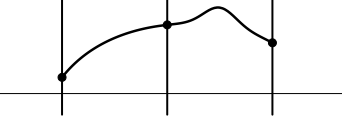
\includegraphics[width=6cm]{Images/proof}};
			\draw [color=black](0,.6) node[anchor=north west] {$l_n(\t_0)$};
			\draw [color=black](-2.4,-1.05) node[anchor=north west] {$\t_0-\delta$};
			\draw [color=black](1.3,-1.05) node[anchor=north west] {$\t_0+\delta$};
			\draw [color=black](-0.3,-1.05) node[anchor=north west] {$\t_0$};
			\end{tikzpicture}
		\end{center}
		Protože $l_n(\t)$ je na~intervalu $(\t_0-\delta,\t_0+\delta)$ diferencovatelná (tedy i~spojitá), pak pro~$\forall\delta$ s~pravděpodobností $\PP_{\t_0}\to1$ existuje $\widehat{\t}_n$ jako řešení $l_n'(\widehat{\t}_n)=0$, které se~nachází v~intervalu $(\t_0-\delta,\t_0+\delta)$ a~je tedy konzistentní pro~$\t_0$.
	\end{proof}
\end{theorem}

\begin{example}[Původně ze~SME]
	Mějme $X_1,...,X_n~iid~\n{\mu,\sigma^2},~\hat{\mu}_\txt{ML}=?,~\widehat{\sigma}^{2}_\txt{ML}=?$
	\[
	\begin{split}
	L(\mu,\sigma^2)&=\prod\limits_{i=1}^n f_{X_i}(x_i,\mu,\sigma^2)=\prod\limits_{i=1}^n \frac{1}{\sqrt{2\pi\sigma^2}}\e{-\frac{(x_i-\mu)^2}{2\sigma^2}}=(2\pi\sigma^2)^{-\frac{n}{2}}\e{-\frac{1}{2\sigma^2}\sumjn(x_j-\mu)^2}.\\
	l(\mu,\sigma^2)&=\ln L(\mu,\sigma^2)=-\frac{n}{2}\ln(2\pi)-\frac{n}{2}\ln\sigma^2 -\frac{1}{2\sigma^2}\sumjn(x_j-\mu)^2.\\
	\frac{\partial l}{\partial \mu}&=\frac{1}{\sigma^2}\sumjn(x_j-\mu)=0\qquad\qquad\qquad\Rightarrow\quad\widehat{\mu}=\frac{1}{n}\sumjn x_j =\oxnn, \\
	\frac{\partial l}{\partial (\sigma^2)}&=-\frac{n}{2}\frac{1}{\sigma^2}+\frac{1}{2\sigma^4}\sumjn(x_j-\mu)^2=0\quad \Rightarrow\quad \widehat{\sigma}^2=\frac{1}{n}\sumjn (x_j-\oxnn)^2.
	\end{split}
	\]
	$$ \frac{\partial^2 l}{\partial\mu^2}=-\frac{n}{\sigma^2},\qquad\frac{\partial^2 l}{\partial\mu\partial\sigma^2}=-\frac{1}{\sigma^4}\sumjn (x_j-\mu),\qquad\frac{\partial^2 l}{\partial(\sigma^2)^2}=\frac{n}{2}\frac{1}{\sigma^4}-\frac{1}{\sigma^6}\sumjn(x_j-\mu)^2, $$
	
	$$ \fisher_{12}=\fisher_{21}=-\EE{ -\frac{1}{\sigma^4}\sumjn (X_j-\mu) }=\frac{1}{\sigma^4} \Br{\sumjn (\underbrace{\E X_j}_{=\mu}-\mu)} =0, $$
	$$  \fisher_{11}=\frac{n}{\sigma^2}, \qquad  \fisher_{22}=-\frac{n}{2}\frac{1}{\sigma^4}+\frac{1}{\sigma^6}\sumjn \underbrace{\E (X_j-\mu)^2}_{\sigma^2}=\frac{n}{2\sigma^4}. $$
	Fisherova informační matice má tedy tvar $\fisher_n=\matice{
		\frac{n}{\sigma^2}}{0}{0}{\frac{n}{2\sigma^4}}=n\matice{
		\frac{1}{\sigma^2}}{0}{0}{\frac{1}{2\sigma^4}}=n\fisher_1(\mu,\sigma^2)$.
	Speciálně pro~odhad jednorozměrného paramentru $\mu$ získáme odhad $\widehat{\mu}_\txt{ML}=\Oxn$, pro~který plyne asymptotická normalita:
	$$ \sqrt{n}(\Oxn-\mu)\Dto \NN(0,\underbrace{\sigma^2}_{\inv{\fisher_1}(\mu)}). $$	
	V případě náhodného výběru z~normálního rozdělení se~tedy jedná o~přesné rozdělení $\Oxn$ (nejenom asymptotické), protože víme, že
	$$ \Oxn\sim\n{\mu,\frac{\sigma^2}{n}},\quad \Oxn-\mu\sim\n{0,\frac{\sigma^2}{n}},\quad \sqrt{n}(\Oxn-\mu)\sim\n{0,\sigma^2}. $$

\end{example}
	\begin{center}
	\begin{tikzpicture}
	\node[inner sep=0pt] (pic) at (0,0)
	{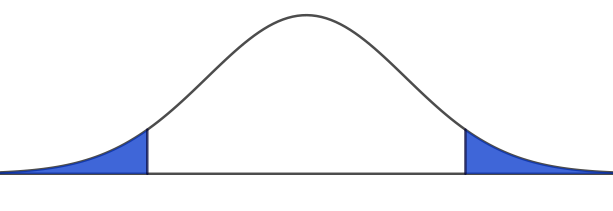
\includegraphics[width=6cm]{Images/KK}};
	\draw [color=black](0.6,1.) node[anchor=north west] {$f_{T^\ast}$};
	\draw [color=blue!40!black](-2.1,-0.75) node[anchor=north west] {$-K_1'$};
	\draw [color=blue!40!black](1.2,-0.75) node[anchor=north west] {$K_1'=u_{1-\frac{\alpha}{2}}$};
	\draw [color=blue!40!black](-2.2,0.2) node[anchor=north west] {$\frac{\alpha}{2}$};
	\draw [color=blue!40!black](1.7,0.2) node[anchor=north west] {$\frac{\alpha}{2}$};
	\end{tikzpicture}
\end{center}